%!TEX TS-program = xelatex
\documentclass[10pt]{article}
\usepackage{amsmath,amssymb,amsfonts} % Typical maths resource packages
\usepackage{float}
\usepackage{graphics}                 % Packages to allow inclusion of graphics
\usepackage{color}                    % For creating coloured text and background
\usepackage{hyperref}
\usepackage{graphicx}                 % For Figures
\usepackage{xepersian}                % For Persian language support


\settextfont{XB Niloofar.ttf}
\hypersetup{
	colorlinks=true,
	linkcolor=blue,
	filecolor=magenta,      
	urlcolor=cyan,
	pdftitle={Overleaf Example},
	pdfpagemode=FullScreen,
}

\begin{document}

\title{بسم اللّه الرحمن الرحیم
	\\[25pt]	پروژه پایانی پردازش زبان طبیعی
}
\author{غزاله محمودی}

\date{\today}
\maketitle
\newpage

\tableofcontents
\newpage

\listoffigures
\newpage

\listoftables
\newpage
	
\section{ 
	\lr{word2vec}
}
در این بخش قصد داریم با استفاده از ماژول gensim بردار
\lr{word2vec}
  را برای هر کلمه حساب کنیم. 

برای به دست آوردن
\lr{word2vec}
 به کمک Gensim تعدادی پارامتر قابل تنظیم دارد که در ادامه به بررسی آن ها می پردازم.

\begin{itemize}
	\item Size 
	
	این پارامتر تعیین کننده سایز vector برای نمایش هر word یا token است. هر چه دیتاست محدود تر و کوچکتر باشد این عدد نیز کوچک تر در نظر گرفته می شود و هر چه دیتاست بزرگتر باشد(کلمات unique بیشتری داشته باشد) باید اندازه vector بزرگتر در نظر گرفته شود. تجربه نشان داده اندازه بین 100 تا 150 برای دیتاست های بزرگ مقدار مناسبی است.
	
	\item Windows 
	
	این پارامتر تعیین کننده بیشترین فاصله مابین کلمه اصلی و همسایه های آن می باشد.از لحاظ تئوری هر چه این سایز کوچکتر باشد کلماتی که بیشتر ارتباط را به یکدیگر دارند به عنوان خروجی برمی گرداند. اگر تعداد داده به اندازه کافی بزرگ باشد سایز پنجره اهمیت زیادی ندارد اما باید این نکته را در نظر گرفت که این سایز نباید خیلی بزرگ یا بیش از حد کوچک باشد. اگر درباره انتخاب آن اطمینان نداریم بهتر است از مقدار پیش فرض استفاده کنیم.
	
	
	\item \lr{Min count}
	
	این پارامتر حداقل تکرار کلمه در دیتاست را نشان می دهد که در صورتی که کلمه ای به این تعداد تکرار شود در
	\lr{word embedding}
	 مورد توجه قرار می گیرد و در غیر این صورت کنار گذاشته می شود. تعیین این عدد در دیتاست های بزرگ برای کنار گذاشتن کلمات کم اهمیت که غالبا کم تکرار می شوند مناسب است. همچنین در مصرف بهینه مموری و حافظه هم تاثیر دارد.
	
	 
	
\end{itemize}

\subsection{بررسی
\lr{bias}
}
در بخش بعدی آزمایش‌ها، احتمال وجود bias در دیتاست مورد بررسی قرار گرفت.
برای این منظور مشابهت‌های مقابل مورد بررسی قرار گرفت.
\begin{flushleft}
\lr{woman as doctor similar as man as ?}
\end{flushleft}

که خروجی به صورت شکل\ref{word2vec-man} شد.

	
\begin{figure}[H]
		\centering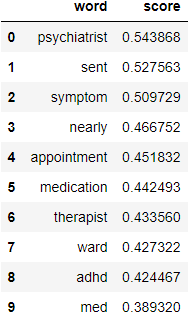
\includegraphics[width=0.3\linewidth]{../reports/word2vec/bias-man.png}
		\caption{ 
			\lr{woman as doctor similar as man as ?}}
		\label{word2vec-man}
	\end{figure}
در ادامه برای پیدا کردن bias احتمالی بین زن و مرد در این دیتاست به ازای ورودی زیر اجرا را تکرار کردیم. خروجی به صورت شکل\ref{word2vec-woman} شد. 
\begin{flushleft}
\lr{man as doctor similar to woman as ?}
\end{flushleft}

	\begin{figure}[H]
	\centering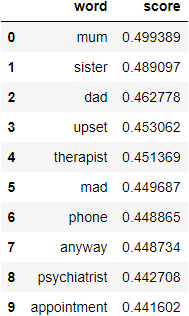
\includegraphics[width=0.3\linewidth]{../reports/word2vec/bias-woman.png}
	\caption{ 
		\lr{man as doctor similar to woman as ?}}
	\label{word2vec-woman}
	\end{figure}

همان‌طور که در گزارشات مطرح شده به وضوح مشخص است این دیتا برای جنسیت خانم‌ها و آقایان bias دارد. در مورد اول اگر شغل زن را دکتر فرض کنیم، مدل برای مرد شغل روان‌پزشک که شاخه‌ای از پزشکی است را انتخاب می‌کند. اما در آزمایش دوم هنگامی که شغل مرد را دکتر در نظر می‌گیریم، برای شعل زن mum را انتخاب می‌کند. گرچه مادری از جایگاه بالایی برخوردار است اما در اینجا نشان‌دهنده bias بر روی جنسیت می‌باشد.

\subsection{بررسی بردار‌های کلمات مشابه  در کلاس‌های مختلف
}

در این بخش بردار‌های کلمات مشترک در دو دسته
\lr{depresion}
و
\lr{happiness}
 را مورد بررسی قرار دادیم. در این آزمایش برای بردار‌ها 
\lr{cosine similarity}
را محاسبه کردیم. اگر دو بردار کاملا یکسان باشند مقدار
\lr{cosine similarity}
برابر با 1 یا نزدیک به 1 می‌شود و در غیر این صورت مقادیر کوچک تر از 1 می‌باشد. نتیجه محاسبه 
\lr{cosine similarity}
برای چند کلمه مشترک بین دسته‌ها به صورت شکل\ref{cosine_similarity} است.

\begin{figure}[H]
	\centering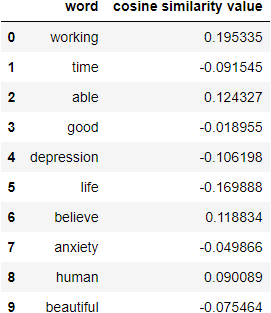
\includegraphics[width=0.5\linewidth]{../reports/word2vec/cosine_similarity.png}
	\caption{ 
		\lr{cosine similarity common words}}
	\label{cosine_similarity}
\end{figure}

همان‌طور که مشخص است اکثر کلمات یکسان در دسته‌های مختلف بردار‌های متفاوتی دارد. دلیل این امر این است که با توجه به context که کلمه در هر کلاس آمده، بردار مورد نظر به دست آمده است. با توجه به اینکه کلمات در متن‌های متفاوتی هستند پس بردار‌های متفاوتی برای آن‌ها وجود دارد.

در ادامه کلمات مشترک کلاس‌های مختلف 
\lr{10 most similarr words}
را برای کلمه life بررسی کردیم و بردار 64 بعدی را در نمودار 2 بعدی نمایش دادیم. 10 کلمه برتر کلاس
\lr{depresion}
در شکل\ref{most_sim_dep} و 10 کلمه برتر کلاس
\lr{happiness}
در شکل\ref{most_sim_hpa} می‌باشد.

\begin{figure}[H]
	\centering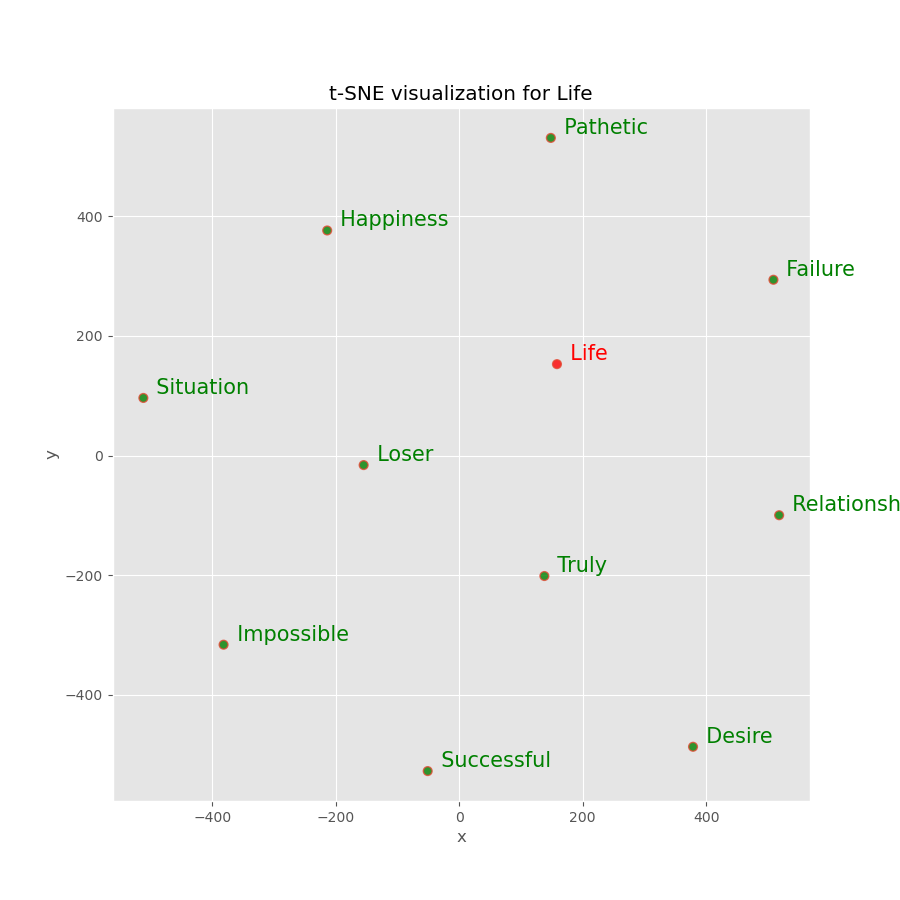
\includegraphics[width=0.6\linewidth]{../reports/word2vec/depression_life_most_similar_word.png}
	\caption{بردار 10 کلمات مشابه 
		\lr{life}}
	\label{most_sim_dep}
\end{figure}

\begin{figure}[H]
	\centering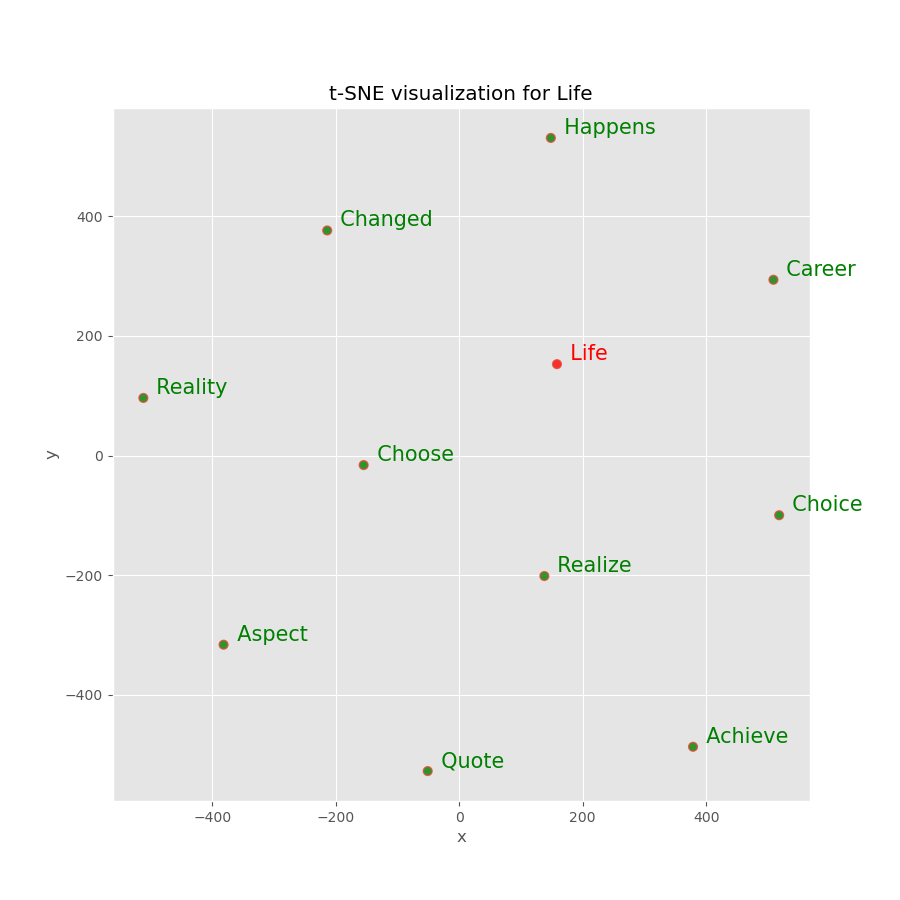
\includegraphics[width=0.6\linewidth]{../reports/word2vec/happiness_life_most_similar_word.png}
	\caption{بردار 10 کلمات مشابه 
		\lr{life}}
	\label{most_sim_hpa}
\end{figure}

\newpage
\section{
	\lr{tokenization}
}

در این قسمت ابتدا پنج 
\lr{vocab size}
برای tokenize کردن داده انتخاب می‌کنیم. دیتا را به پنج بخش تقسیم کرده و در هر مرحله آزمایش، یک بخش به عنوان داده ارزیابی و چهار بخش باقی مانده را به عنوان داده آموزشی در نظر می‌گیریم. به ازای هر
\lr{vocab size}
در این بخش tokenize در مرحله word اجرا می‌شود و  id توکن unk عدد سه در نظر گرفته شده است.	 پنج بار آزمایش انجام می‌دهیم. مدل رت روی داده‌های آموزشی train کرده ودر انتها تعداد توکن‌های unk را به ازای
\lr{vocab size}
های مختلف بر روی داده ارزیابی بررسی می‌کنیم. نتایج به دست آمده در شکل\ref{tok} قابل مشاهده است. 

\begin{figure}[ht!]
	\centering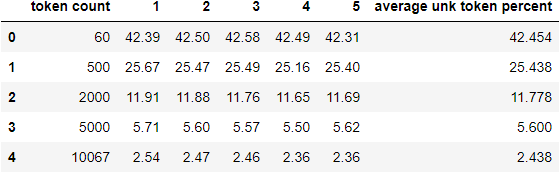
\includegraphics[width=\linewidth]{../reports/tokenization.png}
	\caption{
		\lr{tokenization result}}
	\label{tok}
\end{figure}

همچنین نتایج به صورت متن در
\lr{reports/tokenization.txt}
و log برنامه در 
\lr{logs/tokenization.log}
موجود است. برای اجرا آزمایش‌ها و ذخیره مدل نهایی در پوشه مورد نظر کافیست 
\lr{python3 tokenization.py}
اجرا شود.

همان‌طور که انتظار می‌رفت با افزایش تعداد
\lr{vocab size}
تعداد توکن‌های unk به مقدار قابل توجهی کاهش می‌یابد.
\newpage

\section{
	\lr{parsing}
}

در این قسمت به کمک کد تمرین 3 مدل
\lr{dependency parser}
را بر روی زبان انگلیسی آموزش داده و تعدادی جمله از دیتاست را انتخاب کرده و parse متناظر با آن‌ها را به صورت دستی نوشته و به عنوان فایل تست، قرار می‌دهیم. فایل تست تولید شده در 
\lr{src/parsing/data/project\_data\_test.conll}
قابل مشاهده است (شکل\ref{dep_parser_test}).
\begin{figure}[ht!]
	\centering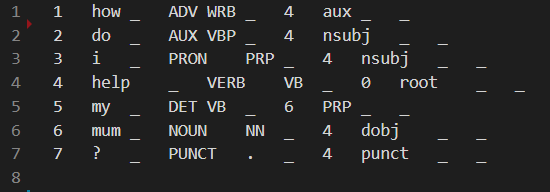
\includegraphics[width=\linewidth]{../reports/dep_parser_test.png}
	\caption{
		\lr{correct dependency parser}}
	\label{dep_parser_test}
\end{figure}

به عنوان مثال مدل برای جمله موجود در شکل\ref{dep_parser} 
\lr{dependency parser}
را به طور کامل درست تشخیص داده است.
\begin{figure}[ht!]
	\centering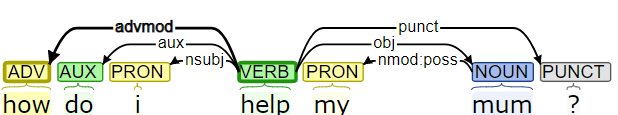
\includegraphics[width=\linewidth]{../reports/dep_parser_1.png}
	\caption{
		\lr{correct dependency parser}}
	\label{dep_parser}
\end{figure}

نکته‌‌ای که در ساخت فایل conll بسیار مهم است و باید بدان توجه شود این است که بین موارد نوشته شده باید یک tab فاصله باشد و در صورت عدم رعایت این فاصله جملات توسط parser به صورت اشتباه خوانده می‌شوند.
\newpage
\section{
	\lr{language model}}
	در این بخش برای آموزش 
	\lr{language model}
	ابتدا داده تمیز را به صورت مناسب آماده می‌کنیم. سپس به ازای هر کدام از دسته‌های 
	\lr{depresion}
	و
	\lr{happiness}
	داده را به شبکه داده تا مدل زبانی آموزش ببیند. در معماری تعریف شده ایتدا یک لایه 
	\lr{embedding}
	قرار داده شده و در ادامه لایه 
	\lr{LSTM}
	با 
	\lr{100 hidden state}
	قرار دارد. لایه دیگری
	\lr{bidirectional LSTM}
	و در ادامه یک لایه dense قرار دارد. لایه انتهایی یک لایه dense با تابع فعال‌سازی softmax می‌باشد که به تعداد همه کلمات موجود نورون دارد. در این لایه به ازای ورودی شبکه مشخص می‌شود چه کلمه باید بعد از عبارت ورودی شبکه بیاید.
	مدل تعریف شده به صورت شکل\ref{lm}
	می‌باشد. دقت و loss برای کلاس‌های مختلف به صورت شکل\ref{lm_dep} و شکل\ref{lm_hap} است. 

	
		\begin{figure}[ht!]
		\centering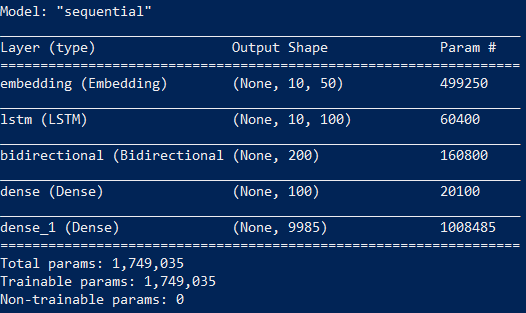
\includegraphics[width=0.8\linewidth]{../reports/lm_model.png}
		\caption{شبکه 
			\lr{language model}}
		\label{lm}
	\end{figure}
	
	
	\begin{figure}[ht!]
		\centering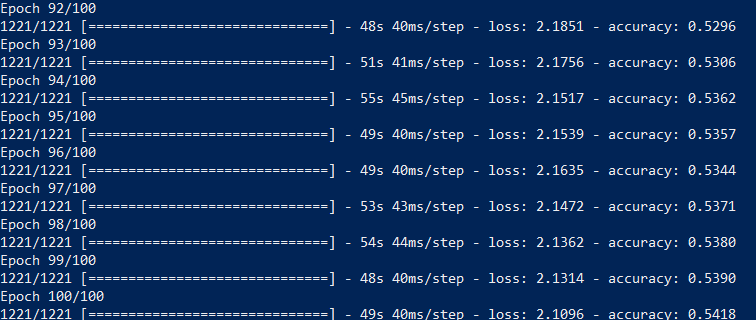
\includegraphics[width=0.9\linewidth]{../reports/lm_dep.png}
		\caption{ 
			\lr{LSTM accuracy and Loss language model on class depression}}
		\label{lm_dep}
	\end{figure}

	\begin{figure}[ht!]
		\centering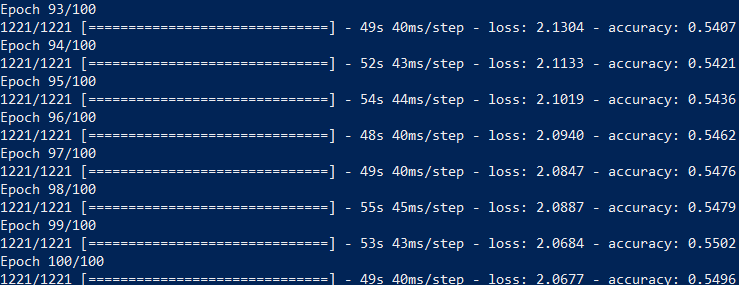
\includegraphics[width=0.9\linewidth]{../reports/lm_hap.png}
		\caption{
			\lr{LSTM accuracy and Loss language model on class happiness}}
		\label{lm_hap}
	\end{figure}

با توجه به حذف stopwords و punctuation از جمله و کم‌بودن دیتا برای آموزش یک مدل زبانی مناسب، مشکلاتی در نحوه جمله بندی و قواعد گرامری جمله ساخته شده توسط مدل وجود دارد. عدم وجود I , am , are و حروف اضافه‌ای همچون is, thst در زمان تمیز کردن دیتا باعث شده چنین جملاتی به وجود بیایند. از طرفی شبکه آموزش دیده pretrain نبوده و برای اولین بار آموزش می بیند و برای آموزش بهتر نیاز به دیتا بسیار بیشتری از حجم دیتا فعلی دارد.

\begin{itemize}
	\item happiness
	
	\lr{take break outside lunch feel like everyone office hate think boring
		since forced office romantic vacation friend friend whole money laying}
	
	\item happiness
	 
	\lr{kill prayed god make accident happen year old relationship family know
		remember im told reminds friend something really eventually wa using}
	
	\item happiness
	
	\lr{i feel so .. like losing grow shell remember hate suck suck fucked cant}
	
	\item depression
	
	\lr{i feel so .. like edgy movie mind hold supportive defense trash sea man}
\end{itemize}

	
\newpage
\section{
	\lr{finu tuning}
}

\subsection{\lr{language model}}
در این بخش با توجه به مطالعات انجام شده بر روی مدل‌های
\lr{GPT2}
 در 
\lr{language model}
و کیفیت خروجی مدل برای این تسک، از
\lr{distilgpt2}
به عنوان مدل pretrain استفاده کرده و مدل را بر دیتاست موجود finetune کردم.

برای اجرا این بخش کافیست
\lr{python3 fine\_tuning.py GPT2}
را اجرا کنید.
به ازای هر کدام از کلاس‌های 
\lr{depresion}
و
\lr{happiness}
مدل را finetune کرده و وزن‌های حاصله به صورت اتوماتیک در
\lr{models/depressionGPT2\_lm}
و
\lr{mosels/happinessGPT2\_lm}
ذخیره می‌شوند. همچنین log در حین اجرا در 
\lr{logs/fine\_tuning\_GPT2.log}
قابل مشاهده هست. نمودار تغییرات  
\lr{loss}
مدل در زمان finetune برای کلاس
\lr{depression}
 به صورت شکل\ref{GPT_dep}
 و برای کلاس
 \lr{happiness}
به صورت شکل\ref{GPT_hap}
می‌باشد.
	\begin{figure}[H]
		\centering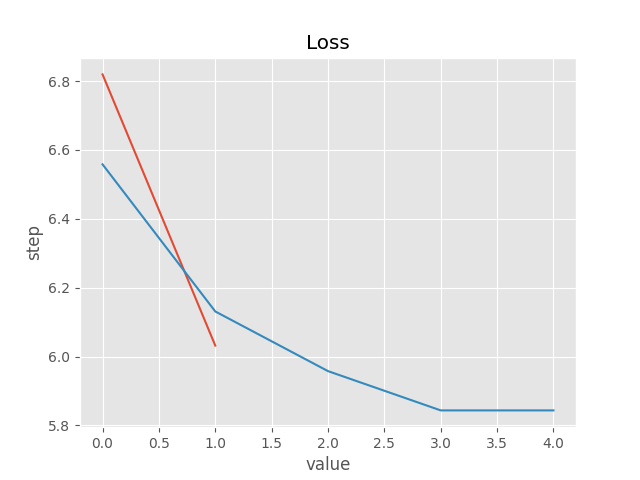
\includegraphics[width=\linewidth]{../reports/loss_history_GPT2_depression.png}
		\caption{ 
			\lr{distilgpt2 Loss language model on class depression}}
		\label{GPT_dep}
	\end{figure}
	
		\begin{figure}[H]
		\centering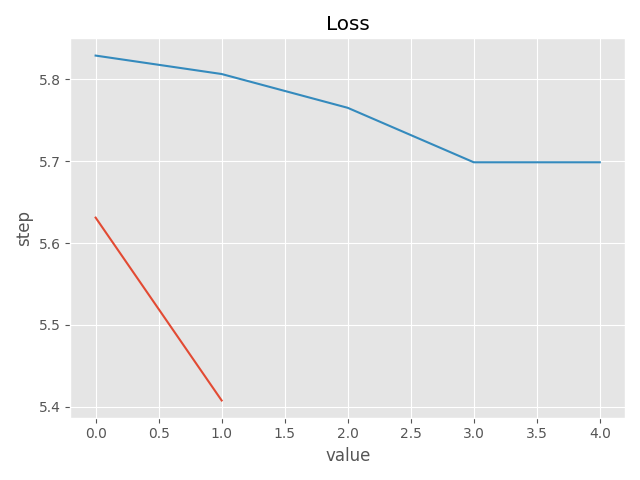
\includegraphics[width=\linewidth]{../reports/loss_history_GPT2_happiness.png}
		\caption{ 
			\lr{distilgpt2 Loss language model on class happiness}}
		\label{GPT_hap}
	\end{figure}


جملات تولید شده با مدل از قبل آموزش دیده
\lr{distilgpt2}
بسیار با کیفیت‌ترو معنی‌دارتر از جملات تولید شده در قسمت قبل می‌باشد.
به ازای هر کدام از کلاس‌ها دو جمله تولید شده که به صورت زیر می‌باشد. نوشته به رنگ آبی توسط مدل تولید شده است.

\begin{itemize}
	\item happiness
	
	\lr{Hi, we have created a success forum for
		since forced office romantic vacation friend friend whole money laying}
	
	
	\item happiness
	
	\lr{Hi, we have created a success forum for}
	\lr{people interested interested    know going want succeed going want fail people want know go past time never successful people want know go past time know succeeding people want know go past time life lived time lived past moment}\color{blue}\\
	
	
	\item happiness
	
	\lr{I'm so depressed. I have nothing to live
		remember im told reminds friend something really eventually wa using}
	
	
	\item depression
	
	\lr{I'm so depressed. I have nothing to live}
	\lr{like edgy movie mind hold supportive defense trash sea man}\color{blue}
\end{itemize}

\subsection{\lr{classification}}
در بخش دوم مدل 
\lr{bert-base-uncased}
از قبل آموزش دیده را برای classification داده‌ها بر روی داده‌های موجود finetune می‌کنیم. 
برای اجرا این بخش کافیست
\lr{python3 fine\_tuning.py Bert}
را اجرا کرد. وزن‌های مدل finetune شده در 
\lr{models/bert\_classification\_lm}
ذخیره می‌شوند. همچنین log در حین اجرا در 
\lr{logs/fine\_tuning\_Bert.log}
می‌باشد. نمودار تغییرات loss در شکل\ref{bert}
قابل مشاهده است.

\begin{figure}[ht!]
	\centering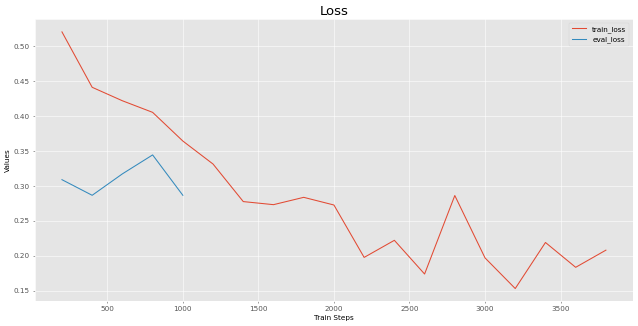
\includegraphics[width=\linewidth]{../reports/loss_history_Bert.png}
	\caption{ 
		\lr{bert-base-uncased Loss classification}}
	\label{bert}
\end{figure}


\newpage

\section{منابع}

\begin{flushleft}
	\url{https://www.kaggle.com/pierremegret/gensim-word2vec-tutorial}
	\url{https://radimrehurek.com/gensim/models/word2vec.html}
	%\url{https://colab.research.google.com/github/google/sentencepiece/blob/master/python/sentencepiece\_python\_module\_example.ipynb#scrollTo=T9BDzLVkUFT4
	\url{https://www.philschmid.de/fine-tune-a-non-english-gpt-2-model-with-huggingface}
	\url{https://machinelearningmastery.com/how-to-develop-a-word-level-neural-language-model-in-keras/}
	\url{https://gmihaila.github.io/tutorial_notebooks/pretrain_transformers_pytorch/}
	\url{https://stackoverflow.com/questions/52277384/calculation-of-cosine-similarity-of-a-single-word-in-2-different-word2vec-models}
\end{flushleft}

\end{document}